% 第5章：加法与数乘、乘法（逐项乘法、矩阵乘法、矩阵幂）、转置与重排、内积、范数与距离、伴随。

\section{加法与数乘}
\label{sec:ls-addition-scaling}

第~\ref{chap:sets-functions-and-proofs}章已经按对应坐标定义了向量、矩阵的逐项相加与实数数乘，第~\ref{sec:ls-vector-spaces}节又把这些规则抽象为线性空间公理。本节不再重复逐项算式，只回答两个实际问题：两个对象或两个映射在什么条件下可以相加，以及按结构组织计算时实际付出多少。

\subsection{定义与性质}

两个数组能够相加，首先要求形状相同、对应索引的含义相同：$\bm A,\bm B\in\mathbb R^{m\times n}$才有$(\bm A+\bm B)_{i,j}=a_{i,j}+b_{i,j}$，向量$\bm x,\bm y\in\mathbb R^d$才有$(\bm x+\bm y)_j=x_j+y_j$。形状不同的数组不能逐项配对；即使元素总数恰好相同，把$m\times n$与$p\times q$直接相加也没有定义，因为第$(i,j)$个位置在两张表中可能记录不同的量。数乘$c\bm A$把每个元素乘以同一个实数$c$，不改变形状。

逐项规则只用到实数加法与乘法，因此第~\ref{sec:ls-vector-spaces}节列出的交换律、结合律、零元与负元、数乘分配律都按位置各自成立，不需要新的验证。需要单独记住的是相容条件：$\bm A+\bm B$合法当且仅当两者属于同一个同型数组空间。

\paragraph{线性组合与张成}
\label{sec:linear-algebra-map-addition}

若干同型对象分别乘以系数后相加，就是它们的\term{线性组合}：$\sum_{j=1}^k c_j\bm A_j$的每个位置是对应位置元素的同一组合。系数$c_j$是实数，不要求非负，也不要求和为$1$；固定一组系数，线性组合把多个记录合并成一个同型记录。

映射也可以叠加。设$T,S:V\to W$是同一对空间之间的两个线性映射，定义
\[
 (aT+bS)(\bm x)=aT\bm x+bS\bm x,\qquad \bm x\in V,
\]
其中$a,b\in\mathbb R$。叠加保持线性：把输入的线性组合代入，两个分支分别展开再汇总即可。在$V$与$W$的固定基下，$T,S$的矩阵为$\bm A,\bm B$，则$aT+bS$的矩阵就是$a\bm A+b\bm B$。

相加的前提是两个映射的定义域与陪域都一致。这并不要求$V=W$：两个从$\mathbb R^2$到$\mathbb R^3$的映射照样可以相加，只是不能与一个从$\mathbb R^3$到$\mathbb R^2$的映射相加。系数$a,b$必须与输入无关；若叠加系数随$\bm x$改变，叠加后的映射一般不再线性，需要单独检验。

\section{乘法}
\label{sec:ls-multiplication}

“相乘”在线性代数里有两种互不相同的含义。逐项乘法在对应位置把两个同形数组配对相乘，不汇总任何索引；矩阵乘法把两个映射经中间空间复合，对被消去的索引求和。二者输入条件、输出形状和线性性都不同。同一个方阵与自身反复复合得到矩阵幂，它是矩阵乘法的特例，放在本节最后。

\subsection{逐项乘法}

\subsubsection{定义与性质}

\paragraph{逐项乘积（Hadamard积）}

设$\bm A,\bm B\in\mathbb R^{m\times n}$，\term{逐元素乘积}（Hadamard product）记作$\bm A\odot\bm B$，定义为
\begin{equation}
 (\bm A\odot\bm B)_{i,j}=a_{i,j}b_{i,j},
 \label{eq:ls-hadamard}
\end{equation}
输出仍是$m\times n$，每个位置只取两个因子在同一位置的数相乘，不对任何索引求和。例如
\[
 \begin{bmatrix}1&2\\3&4\end{bmatrix}
 \odot
 \begin{bmatrix}0&1\\1&0\end{bmatrix}
 =
 \begin{bmatrix}0&2\\3&0\end{bmatrix}.
\]
它适合表达“用一个掩码挑选或调制另一个数组”：固定掩码$\bm M$后，$\bm X\mapsto\bm M\odot\bm X$把$\bm M$为零的位置置零，把非零位置按系数缩放。

由于等式~\eqref{eq:ls-hadamard} 右端只是实数乘法，按位置逐项验证即得交换律$\bm A\odot\bm B=\bm B\odot\bm A$、结合律$(\bm A\odot\bm B)\odot\bm C=\bm A\odot(\bm B\odot\bm C)$，以及对加法的分配律$\bm A\odot(\bm B+\bm C)=\bm A\odot\bm B+\bm A\odot\bm C$；单位元是全$1$数组。固定一个因子时$\bm X\mapsto\bm M\odot\bm X$是线性映射；两个因子都作为未知量时，乘积只对各自分别线性：同时把两者放大两倍，结果放大四倍。

逐项乘积不是映射复合。上面两个矩阵的普通乘积是$\begin{smallmatrix}2&1\\4&3\end{smallmatrix}$，与逐项结果完全不同。逐项乘法还依赖所选坐标：换基后同一对象的坐标改变，原掩码位置不再对应原来的方向。因此它描述的是记录层面的配对，而矩阵乘法对应与坐标无关的映射复合。

\subsection{矩阵乘法}

\subsubsection{定义与含义}

矩阵乘法来自映射的复合。设$T:U\to V$、$S:V\to W$是线性映射，先让$\bm x$经过$T$得到中间结果$\bm y=T\bm x\in V$，再让$S$作用于$\bm y$，得到$S(T\bm x)\in W$。复合$S\circ T$从$U$直接到$W$，中间空间$V$只用于衔接。

在固定基下设$\bm y=\bm B\bm x$（$\bm B\in\mathbb R^{d\times k}$），$\bm z=\bm A\bm y$（$\bm A\in\mathbb R^{m\times d}$）。逐坐标展开
\[
 z_i=\sum_{\ell=1}^d a_{i,\ell}y_\ell
 =\sum_{\ell=1}^d a_{i,\ell}\sum_{j=1}^k b_{\ell,j}x_j
 =\sum_{j=1}^k\left(\sum_{\ell=1}^d a_{i,\ell}b_{\ell,j}\right)x_j.
\]
有限求和交换次序后，中间坐标$y_\ell$被消去，$z_i$直接由$x_j$表示。

\paragraph{矩阵乘法的定义}

对相容形状的$\bm A\in\mathbb R^{m\times d}$、$\bm B\in\mathbb R^{d\times k}$，乘积$\bm A\bm B\in\mathbb R^{m\times k}$定义为
\begin{equation}
 (\bm A\bm B)_{i,j}=\sum_{\ell=1}^d a_{i,\ell}b_{\ell,j}.
 \label{eq:linear-algebra-matrix-product}
\end{equation}
左矩阵的列数必须等于右矩阵的行数，这个公共维数就是被消去的中间空间维数；第$(i,j)$项取左矩阵第$i$行与右矩阵第$j$列逐项相乘再相加。按行乘列不是任意约定，而是“先代入再读出”这一复合要求的唯一写法。

同一乘积有三种读法。按列看，$(\bm A\bm B)_{:,j}=\bm A\bm B_{:,j}$：$\bm A$作用在$\bm B$的每一列上，乘积记录$\bm B$的各列再经$\bm A$传播的结果。按行看，$(\bm A\bm B)_{i,:}=\bm A_{i,:}\bm B$：$\bm B$作用在$\bm A$的每一行上。按中间索引看，
\begin{equation}
 \bm A\bm B=\sum_{\ell=1}^d\bm A_{:,\ell}\bm B_{\ell,:},
 \label{eq:ls-product-outer-sum}
\end{equation}
乘积是$d$个秩一矩阵之和，每个中间维度贡献一项。三种读法给出同一组数，区别在于先汇总哪个索引，这决定了后面的分块与近似方式。

规则$\bm x\mapsto\bm A\bm x+\bm b$在$\bm b\neq\bm0$时是仿射映射而不是线性映射，因为它把$\bm0$送到$\bm b$。两个仿射映射$\bm x\mapsto\bm A_1\bm x+\bm b_1$、$\bm y\mapsto\bm A_2\bm y+\bm b_2$复合得$\bm x\mapsto\bm A_2\bm A_1\bm x+(\bm A_2\bm b_1+\bm b_2)$，平移项也被后一个映射作用。给坐标补一个恒为$1$的末位，仿射映射可以写成增广空间上的线性作用：
\begin{equation}
 \begin{bmatrix}\bm A&\bm b\\ \bm0^\top&1\end{bmatrix}
 \begin{bmatrix}\bm x\\1\end{bmatrix}
 =
 \begin{bmatrix}\bm A\bm x+\bm b\\1\end{bmatrix}.
 \label{eq:ls-affine-homogeneous}
\end{equation}
大矩阵对整个增广空间是线性的，但原输入被限制在末坐标为$1$的集合上，不能据此声称原映射线性；复合仿射映射对应增广矩阵的普通乘积。

\subsubsection{运算性质}
\label{sec:linear-algebra-map-composition}

映射复合满足结合律：$(R\circ S)\circ T$与$R\circ(S\circ T)$都是先$T$、再$S$、后$R$。翻译成矩阵即$(\bm A\bm B)\bm C=\bm A(\bm B\bm C)$，可在式~\eqref{eq:linear-algebra-matrix-product} 中交换有限求和次序验证，所以多个相容矩阵连乘不需要规定括号。复合也保持叠加：$\bm A(\bm B+\bm C)=\bm A\bm B+\bm A\bm C$，$(\bm A+\bm B)\bm C=\bm A\bm C+\bm B\bm C$，$c(\bm A\bm B)=(c\bm A)\bm B=\bm A(c\bm B)$。单位矩阵满足$\bm I_m\bm A=\bm A=\bm A\bm I_d$，对应恒等映射。

复合次序不能交换。先交换坐标再保留第一坐标，与先保留第一坐标再交换，结果不同：
\[
 \begin{bmatrix}1&0\\0&0\end{bmatrix}
 \begin{bmatrix}0&1\\1&0\end{bmatrix}
 =
 \begin{bmatrix}0&1\\0&0\end{bmatrix},\qquad
 \begin{bmatrix}0&1\\1&0\end{bmatrix}
 \begin{bmatrix}1&0\\0&0\end{bmatrix}
 =
 \begin{bmatrix}0&0\\1&0\end{bmatrix}.
\]
一般$\bm A\bm B\neq\bm B\bm A$，书写乘积时必须从右向左读作用顺序。

乘积可以为零而两个因子都不为零：取$\bm A=\begin{smallmatrix}1&0\\0&0\end{smallmatrix}$、$\bm B=\begin{smallmatrix}0&0\\1&0\end{smallmatrix}$，则$\bm A\bm B=\bm0$。$\bm A\bm B=\bm0$恰好意味着$\bm B$的每一列都落入$\bm A$的零空间，即$\operatorname{range}(\bm B)\subseteq\operatorname{null}(\bm A)$：右因子的可达方向被左因子完全消去，因此不能由$\bm A\bm B=\bm0$推出某个因子为零。

把矩阵按行、列分成尺寸相容的小块，乘法规则对块照样成立：$\bm C_{i,j}=\sum_\ell\bm A_{i,\ell}\bm B_{\ell,j}$，其中$\bm A_{i,\ell}$的列数须等于$\bm B_{\ell,j}$的行数。例如把中间维数分成两段，$\bm C_{i,j}=\bm A_{i,1}\bm B_{1,j}+\bm A_{i,2}\bm B_{2,j}$，与整段求和逐项相等。这称为分块矩阵乘法，块可以像数一样参与运算，只是块之间的次序不能交换。

由第~\ref{sec:ls-injective-surjective-invertible}节的可逆判定，方阵乘积$\bm A\bm B$可逆当且仅当$\bm A$与$\bm B$都可逆，且$(\bm A\bm B)^{-1}=\bm B^{-1}\bm A^{-1}$：先作用的后撤销。

\subsection{矩阵幂}
\label{sec:ls-matrix-powers}
\label{sec:ch06-powers-spectrum}

同一个方阵反复作用，是矩阵乘法最常见的特例：定常迭代$\bm x^{(k+1)}=\bm A\bm x^{(k)}$走$k$步后得到$\bm x^{(k)}=\bm A^k\bm x^{(0)}$。

\paragraph{定义与运算规则}

矩形矩阵不能与自身复合，幂只对$d$阶方阵定义：$\bm A^k$是$k$个$\bm A$连乘（$k\geq1$），并规定$\bm A^0=\bm I_d$，表示不施加任何作用；$\bm A$可逆时再定义负幂$\bm A^{-k}=(\bm A^{-1})^k$。幂是作用的反复复合，不是逐元素乘方：$\bm A=\begin{pmatrix}1&1\\0&1\end{pmatrix}$给出$\bm A^2=\begin{pmatrix}1&2\\0&1\end{pmatrix}$，非对角元随复合次数累加。

由结合律，同一矩阵的幂满足$\bm A^m\bm A^n=\bm A^{m+n}$、$(\bm A^m)^n=\bm A^{mn}$（指数在有定义的范围内取整数），不同次幂彼此交换。不同矩阵则不然：$(\bm B\bm C)^2=\bm B\bm C\bm B\bm C$只有在$\bm B\bm C=\bm C\bm B$时才能整理成$\bm B^2\bm C^2$。例如$\bm B=\begin{pmatrix}0&1\\0&0\end{pmatrix}$、$\bm C=\begin{pmatrix}1&0\\1&0\end{pmatrix}$给出$(\bm B\bm C)^2=\begin{pmatrix}1&0\\0&0\end{pmatrix}$，而$\bm B^2\bm C^2=\bm0$。

两类幂关系经常出现。满足$\bm A^2=\bm A$的作用称为\term{幂等}（idempotent），施加一次与施加多次效果相同，把向量投到某个子空间上的投影就是这种作用。存在正整数$s$使$\bm N^s=\bm0$的作用称为\term{幂零}（nilpotent），它在有限步后把所有向量送到零；例如$\bm N=\begin{pmatrix}0&1\\0&0\end{pmatrix}\neq\bm0$，却有$\bm N^2=\bm0$。

\paragraph{特征值与特征向量}
\label{sec:matrix-analysis-spectrum}

直接连乘会不断混合坐标，$\bm A^k$的长期样子难以从元素看出。第~\ref{sec:ls-operator-eigenvectors}节的特征向量给出简化：
由$\bm A\bm v=\lambda\bm v$归纳得$\bm A^k\bm v=\lambda^k\bm v$，沿特征方向，$k$次作用化为标量乘方，长度乘以$|\lambda|^k$，
$\lambda<0$时每次还翻转方向。例如$\bm A=\begin{pmatrix}0.8&4\\0&0.5\end{pmatrix}$满足$\bm A(1,0)^\top=0.8(1,0)^\top$与
$\bm A(-40/3,1)^\top=0.5(-40/3,1)^\top$，两条特征方向上的分量分别按$0.8^k$与$0.5^k$衰减。

若$\bm A$实可对角化，把$d$个线性无关的特征向量排成可逆矩阵$\bm V$，则$\bm A\bm V=\bm V\bm\Lambda$，即
$\bm A=\bm V\bm\Lambda\bm V^{-1}$，其中$\bm\Lambda$是特征值组成的对角矩阵；于是$\bm A^k=\bm V\bm\Lambda^k\bm V^{-1}$，
幂只需对对角元逐个乘方。并非每个实方阵都可对角化：$\begin{pmatrix}0.8&1\\0&0.8\end{pmatrix}$的特征向量只有$(1,0)^\top$的倍数，
凑不出两条独立方向，其幂中会出现$k\,0.8^{k-1}$这样的项。特征值怎样求出、何时可以对角化，要借助第~\ref{sec:ls-determinant-properties}节的行列式回答。

\section{转置与重排}
\label{sec:ls-reshaping}
\label{sec:linear-algebra-tensors-structured-operations}

加法与乘法都产生新的数值；还有一类操作只改变元素记录在哪个位置，不对任何索引求和，也不改变元素数值。转置、轴置换、reshape与向量化都属于这一类，使用前必须说清新索引怎样对应旧索引。

\subsection{索引变换}

转置交换行与列：若$\bm A\in\mathbb R^{m\times n}$，则$\bm A^\top\in\mathbb R^{n\times m}$满足$(\bm A^\top)_{j,i}=a_{i,j}$。每个元素原样搬到新位置，形状交换而数值不变。

对多于两个轴的数组，\term{维度重排}（permutation of axes）按给定顺序调换轴的位置。例如$y_{i,k,j}=x_{i,j,k}$把$b\times\ell\times d$的数组变为$b\times d\times\ell$：第一个轴保持原位，第二、第三轴互换。元素跟随自己的索引移动，轴的含义不变，只是记录次序改变。

\term{形状重整}（reshape）先指定元素的遍历顺序，再把同一个数列装入另一形状，仅要求元素总数相同。以
$\bm A=\begin{smallmatrix}1&2&3\\4&5&6\end{smallmatrix}$为例，轴交换得到
$\bm A^\top=\begin{smallmatrix}1&4\\2&5\\3&6\end{smallmatrix}$，而按行读取后重整成$3\times2$得到
$\begin{smallmatrix}1&2\\3&4\\5&6\end{smallmatrix}$，两者不同。所以重整不能只给目标形状，还要给遍历顺序；形状相同不能说明完成了轴交换。

图~\ref{fig:vol1-add-linear-transpose-reshape} 把两种结果并排放置：转置后原两行分别成为两列，按行重整则把数列$1,2,3,4,5,6$依次装入新表，原来相邻的元素被安排到不同位置。
\begin{figure}[!htb]
  \centering
  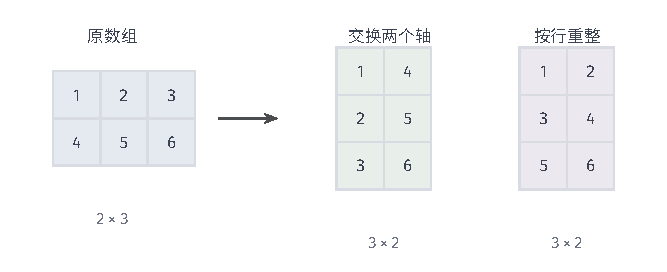
\includegraphics[width=112mm]{figures/01-mathematical-preliminaries-upper/02-linear-spaces/tikz/comprehension-additions/linear-transpose-reshape.pdf}
  \caption{轴交换与按行重整。原数组两行为$(1,2,3)$与$(4,5,6)$；中图转置后两列分别保留原来的两行，右图则把按行读取的数列$1,2,3,4,5,6$依次装入$3\times2$数组。数字及其排列由正文示例直接给出。}
  \label{fig:vol1-add-linear-transpose-reshape}
\end{figure}

\paragraph{向量化}

按列堆叠的\term{向量化}（vectorization）把$m\times n$矩阵展成长列：
\[
 \operatorname{vec}(\bm A)=(a_{1,1},\ldots,a_{m,1},a_{1,2},\ldots,a_{m,n})^\top,
\]
元素$a_{i,j}$对应一维索引$i+(j-1)m$。反过来，矩阵展开（unfolding）把多维数组的指定轴选为行、其余轴合并为列，得到一个矩阵；选哪些轴保留为独立索引，决定展开结果的形状，也决定后续乘积汇总哪个轴。向量化与展开都是固定索引映射的reshape，保留全部信息。

\subsection{运算性质}

目标形状与遍历顺序固定后，转置、轴置换、reshape与向量化都是数组空间之间的线性双射：它们把加法和数乘逐项搬到新排列，逆变换（再转置一次、逆置换、按原次序装回）恢复原数组。因此$(\bm A+\bm B)^\top=\bm A^\top+\bm B^\top$、$(c\bm A)^\top=c\bm A^\top$一类等式按位置直接成立。

转置与乘法的交互由元素公式推出：
\[
 (\bm A^\top)^\top=\bm A,\qquad
 (\bm A\bm B)^\top=\bm B^\top\bm A^\top,\qquad
 (\bm A^{-1})^\top=(\bm A^\top)^{-1}.
\]
乘积转置后因子次序反转；可逆矩阵转置后仍可逆，逆与转置可交换次序。转置还保持矩阵秩，因为行空间与列空间只是互换。一般reshape不保持矩阵秩：它只重排元素，新矩阵各行各列之间的线性相关关系可以完全不同。轴置换与reshape都不是映射作用，把存储格式当成几何性质或变换效果，是这里最常见的错误。

\section{内积}
\label{sec:ls-inner-products}

加法与乘法回答怎样合并对象，内积则把两个对象配成一个标量：它同时给出长度、角度和垂直的判据。第~\ref{chap:sets-functions-and-proofs}章已在标准坐标下定义$\langle\bm x,\bm y\rangle=\sum_j x_jy_j$，本节先把它抽象为配对公理，再引入区分方向代价的加权配对，最后用Gram矩阵建立正交分解和线性泛函的内积表示。

\subsection{内积的定义与性质}

\paragraph{内积的定义}

\begin{definition}[实内积]
\label{def:linear-algebra-inner-product}
\label{def:functional-inner-product-space}
实向量空间$V$上的\term{内积}（inner product）是映射$\langle\cdot,\cdot\rangle:V\times V\to\mathbb R$，同时满足下列三条公理。
\begin{enumerate}
 \item 双线性：对两个变量分别保持线性组合，即$\langle a\bm x+b\bm y,\bm z\rangle=a\langle\bm x,\bm z\rangle+b\langle\bm y,\bm z\rangle$，且对第二变量同样线性。
 \item 对称性：$\langle\bm x,\bm y\rangle=\langle\bm y,\bm x\rangle$。
 \item 正定性：$\langle\bm x,\bm x\rangle>0$对所有非零$\bm x$成立，且$\langle\bm x,\bm x\rangle=0$当且仅当$\bm x=\bm0$。
\end{enumerate}
配备内积的向量空间称为\term{内积空间}（inner-product space）。
\end{definition}

标准实坐标的内积是$\langle\bm x,\bm y\rangle=\bm x^\top\bm y=\sum_j x_jy_j$。由配对直接诱导长度
\begin{equation}
 \lVert\bm x\rVert=\sqrt{\langle\bm x,\bm x\rangle},
 \label{eq:linear-algebra-inner-product-norm}
\end{equation}
$\langle\bm x,\bm y\rangle=0$时称两向量\term{正交}（orthogonal）。

\paragraph{Cauchy--Schwarz不等式}

内积能否给出夹角，取决于配对值是否受两个长度控制。
\begin{theorem}[Cauchy--Schwarz不等式]
\label{thm:linear-algebra-cauchy-schwarz}
在内积空间中，$|\langle\bm x,\bm y\rangle|\leq\lVert\bm x\rVert\,\lVert\bm y\rVert$，等号成立当且仅当两向量线性相关。
\end{theorem}
\begin{proof}
$\bm y=\bm0$时两边都为零。否则令$a=\langle\bm x,\bm y\rangle/\lVert\bm y\rVert^2$，则
\[
 0\leq\lVert\bm x-a\bm y\rVert^2
 =\lVert\bm x\rVert^2-\frac{\langle\bm x,\bm y\rangle^2}{\lVert\bm y\rVert^2}.
\]
移项即得不等式；等号恰好要求$\bm x-a\bm y=\bm0$，即两向量共线。
\end{proof}

非零向量的夹角由$\cos\theta=\langle\bm x,\bm y\rangle/(\lVert\bm x\rVert\lVert\bm y\rVert)$定义，CS不等式保证它落在$[-1,1]$。例如$\bm x=(1,0)^\top$、$\bm y_\varepsilon=(1,\varepsilon)^\top$随$\varepsilon\to0$趋近共线，
\begin{equation}
 \cos\theta_\varepsilon=\frac{1}{\sqrt{1+\varepsilon^2}}\longrightarrow1,
 \label{eq:linear-algebra-nearly-collinear-angle}
\end{equation}
这给“几乎同向”一个确定的欧氏度量；更换内积也会更换角度。

并非每个范数都来自内积。实向量空间中一个范数来自内积，当且仅当它满足\term{平行四边形恒等式}
\begin{equation}
 \lVert\bm x+\bm y\rVert^2+\lVert\bm x-\bm y\rVert^2
 =2\lVert\bm x\rVert^2+2\lVert\bm y\rVert^2.
 \label{eq:functional-parallelogram-identity}
\end{equation}
必要性由内积展开直接得到；例如第~\ref{sec:ls-norms-distances}节的$\ell_1$范数在$\bm e_1,\bm e_2$上左侧为$8$、右侧为$4$，故不来自任何内积。充分性可用极化公式$\langle\bm x,\bm y\rangle=(\lVert\bm x+\bm y\rVert^2-\lVert\bm x-\bm y\rVert^2)/4$恢复配对，这里不展开。

对同形矩阵，把元素看作有限坐标，得到\term{Frobenius内积}
\[
 \langle\bm A,\bm B\rangle_{\mathrm F}=\sum_{i,j}a_{i,j}b_{i,j},
 \qquad
 \lVert\bm A\rVert_{\mathrm F}=\left(\sum_{i,j}a_{i,j}^2\right)^{1/2}.
\]
这是矩阵作为数表本身的长度；它与矩阵作为变换时的最大放大率不是同一口径，后者在第~\ref{sec:ls-matrix-norms}节建立。

\subsection{加权内积}
\label{sec:ls-weighted-inner-products}

标准坐标把每个方向一视同仁，但实际问题里不同方向的代价不同。设$\bm M=\operatorname{diag}(4,1)$，则$\sqrt{4x_1^2+x_2^2}$把第一坐标的偏差放大两倍：点$(1,1)$的欧氏长度是$\sqrt2$，这种加权长度却是$\sqrt5$。只要权重矩阵满足适当条件，这样的长度仍来自一个合法内积。

对称矩阵$\bm M$给出二次型$q(\bm x)=\bm x^\top\bm M\bm x$：若对每个非零$\bm x$都有$q(\bm x)>0$，称$\bm M$\term{正定}（positive definite）；若只保证$q(\bm x)\geq0$，称$\bm M$\term{半正定}（positive semidefinite）。要求对称，是因为配对必须对称；非对称部分在$\bm x^\top\bm M\bm x$中自动抵消，不进入二次型。

\paragraph{加权内积的定义}

对称正定$\bm M$给出加权配对
\[
 \langle\bm x,\bm y\rangle_{\bm M}=\bm x^\top\bm M\bm y,
 \qquad
 \lVert\bm x\rVert_{\bm M}=\sqrt{\bm x^\top\bm M\bm x}.
\]
它满足双线性、对称与正定性，是一个合法内积。若$\bm M$仅半正定，配对只给半内积，诱导半范数以及伪距离
\begin{equation}
 d_{\bm M}(\bm x,\bm y)
 =\sqrt{(\bm x-\bm y)^\top\bm M(\bm x-\bm y)}.
 \label{eq:linear-algebra-mahalanobis-pseudodistance}
\end{equation}
不同点的距离可能为零：例如$\bm M=\operatorname{diag}(1,0)$无法区分$(0,0)^\top$与$(0,1)^\top$。半正定时CS不等式仍可由$\langle\bm x+t\bm y,\bm x+t\bm y\rangle_{\bm M}\geq0$对所有实数$t$成立得到，三角不等式保留。

\paragraph{Gram因子定理}

加权配对不必当作新几何：有限维半正定矩阵都能写成欧氏平方和。
\begin{theorem}[半正定矩阵的配方因子]
\label{thm:ls-gram-factor}
设$\bm M\in\mathbb R^{r\times r}$对称半正定，则存在$\bm L$使$\bm M=\bm L^\top\bm L$；若$\bm M$正定，可取$\bm L$可逆。
\end{theorem}
\begin{proof}
对$r$归纳。$r=1$时$\bm M=(m_{1,1})$且$m_{1,1}\geq0$，取$\bm L=(\sqrt{m_{1,1}})$即可。

若所有对角项都为零，任取$i,j$，把$\bm x=\bm e_i+t\bm e_j$代入半正定性：
\[
 0\leq\bm x^\top\bm M\bm x=2t\,m_{i,j}+t^2m_{j,j}=2t\,m_{i,j},
\]
对正负$t$同时成立迫使$m_{i,j}=0$，于是$\bm M=0$，取$\bm L=0$。

否则存在正对角项。取一个置换矩阵$\bm P$（行列同步交换，$\bm P^\top=\bm P^{-1}$）把它换到首位，记
\[
 \widetilde{\bm M}=\bm P\bm M\bm P^\top
 =\begin{bmatrix}a&\bm b^\top\\ \bm b&\bm C\end{bmatrix},\qquad a>0.
\]
配方消去第一行：令$\bm x=(-\bm b^\top\bm u/a,\bm u)$，则$\bm x^\top\widetilde{\bm M}\bm x=\bm u^\top(\bm C-\bm b\bm b^\top/a)\bm u\geq0$，故余项$\bm M'=\bm C-\bm b\bm b^\top/a$仍半正定。由归纳假设$\bm M'=\bm L'^\top\bm L'$，取上三角因子
\[
 \widetilde{\bm L}=\begin{bmatrix}\sqrt a&\bm b^\top/\sqrt a\\ \bm0&\bm L'\end{bmatrix},
\]
直接相乘得
\[
 \widetilde{\bm L}^\top\widetilde{\bm L}
 =\begin{bmatrix}a&\bm b^\top\\ \bm b&\bm b\bm b^\top/a+\bm L'^\top\bm L'\end{bmatrix}
 =\widetilde{\bm M}.
\]
换回原矩阵：$\bm M=\bm P^\top\widetilde{\bm M}\bm P=(\widetilde{\bm L}\bm P)^\top(\widetilde{\bm L}\bm P)$，取$\bm L=\widetilde{\bm L}\bm P$即可。

正定时$\bm M'$也正定（上述$\bm x$在$\bm u\neq\bm0$时非零），归纳得$\bm L'$可逆，于是$\widetilde{\bm L}$可逆，$\bm L=\widetilde{\bm L}\bm P$仍可逆。
\end{proof}
于是加权长度可写成$\lVert\bm x\rVert_{\bm M}=\lVert\bm L\bm x\rVert_2$：正定时只是换了一组坐标，退化时则把$\bm L$的零空间方向压成零长度。使用半内积前必须先说明哪些方向被忽略，不能把退化配对当成正定内积参与正交判断。证明中的配方步骤就是第~\ref{sec:ls-exact-linear-equations}节Cholesky分解的雏形。

对两个对称矩阵记$\bm M\succeq\bm N$当且仅当$\bm M-\bm N$半正定，即$\bm x^\top\bm M\bm x\geq\bm x^\top\bm N\bm x$对所有$\bm x$成立，它给出加权长度的逐点比较$\lVert\bm x\rVert_{\bm M}\geq\lVert\bm x\rVert_{\bm N}$。作可逆线性替换$\bm x=\bm S\bm z$，二次型变为$\bm z^\top(\bm S^\top\bm M\bm S)\bm z$；这种合同变换$\bm M\mapsto\bm S^\top\bm M\bm S$保持半正定性、正定性与序关系。因此换基后新坐标下的度量矩阵是$\bm S^\top\bm M\bm S$而不是$\bm M$，把新坐标直接按欧氏长度比较，一般已经换了问题。

\subsection{正交关系}
\label{sec:ls-orthogonality}

\paragraph{Gram矩阵}

正交是两个向量之间的关系；一组向量之间的全部配对关系由一张数表记录。
\begin{definition}[有限向量族的Gram矩阵]
\label{def:linear-algebra-gram-matrix}
向量$\bm b_1,\ldots,\bm b_r$的\term{Gram矩阵}（Gram matrix）为$g_{i,j}=\langle\bm b_i,\bm b_j\rangle$。若$\bm B$以它们为列，标准坐标中$\bm G=\bm B^\top\bm B$，加权坐标中$\bm G=\bm B^\top\bm M\bm B$。
\end{definition}

因为$\bm a^\top\bm G\bm a=\lVert\sum_j a_j\bm b_j\rVert^2\geq0$，Gram矩阵半正定；并且$\bm G$正定（从而非奇异）当且仅当这组向量线性无关：线性相关时某个非零系数使组合为零，平方长度为零；线性无关时任意非零系数的组合非零，平方长度为正。$\bm G$是对角阵恰好表示这组向量两两正交，是单位阵则表示两两正交且长度为$1$。图~\ref{fig:ls-gram-matrix-coefficients} 把两条基向量的两两内积排成数表。
\begin{figure}[!htb]
  \centering
  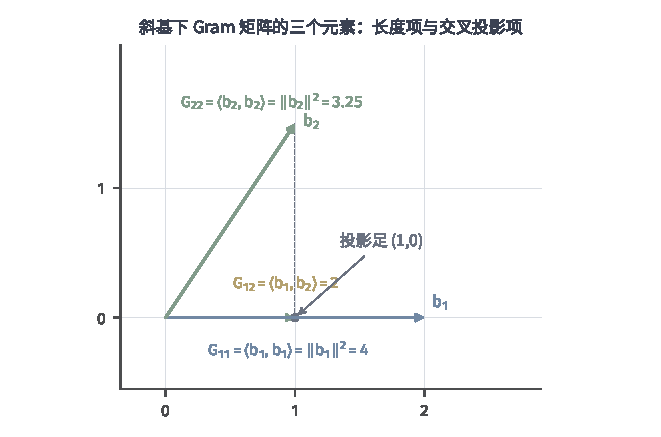
\includegraphics[width=112mm]{figures/01-mathematical-preliminaries-upper/02-linear-spaces/matplotlib/ls-gram-matrix-coefficients/ls-gram-matrix-coefficients.pdf}
  \caption{Gram矩阵把一组基向量的两两内积排成数表。左：平面上两条不垂直的基向量$\bm b_1,\bm b_2$及其夹角；右：$G_{i,j}=\langle\bm b_i,\bm b_j\rangle$构成的$2\times2$Gram矩阵，对角元为各向量长度平方，非对角元为夹角投影。基越接近正交，非对角元越接近零；线性相关时$\det\bm G=0$。向量与矩阵均为解析教学例。}
  \label{fig:ls-gram-matrix-coefficients}
\end{figure}

\paragraph{正交补与正交直和}

设$U$是有限维内积空间$V$的子空间，\term{正交补}（orthogonal complement）定义为
\[
 U^\perp=\{\bm r\in V:\langle\bm u,\bm r\rangle=0,\ \forall\bm u\in U\}.
\]
Gram矩阵非奇异给出正交分解的存在与唯一。
\begin{lemma}[正交直和]
\label{lem:ls-orthogonal-decomposition}
设$U$是有限维内积空间$V$的子空间，则每个$\bm x\in V$唯一分解为$\bm x=\bm u+\bm r$，其中$\bm u\in U$、$\bm r\in U^\perp$；即$V=U\oplus U^\perp$。
\end{lemma}
\begin{proof}
取$U$的一组基$\bm b_1,\ldots,\bm b_r$，其Gram矩阵$\bm G$非奇异。对任意$\bm x$，令$\bm u=\sum_j a_j\bm b_j$，并要求$\bm r=\bm x-\bm u$与每个$\bm b_i$正交，得到系数方程
\[
 \sum_j g_{i,j}a_j=\langle\bm b_i,\bm x\rangle,\qquad i=1,\ldots,r,
\]
即$\bm G\bm a=(\langle\bm b_i,\bm x\rangle)_i$。非奇异$\bm G$保证系数唯一解出，残差$\bm r$与全部基向量正交，因而落在$U^\perp$。

若$\bm x=\bm u+\bm r=\bm u'+\bm r'$是两种分解，则$\bm u-\bm u'=\bm r'-\bm r$同时属于$U$与$U^\perp$，与自身正交，长度为零，故两种分解相同。
\end{proof}
这里只证明正交分量存在且唯一；它就是$U$中离$\bm x$最近的点，这一判定与具体算法在第~\ref{sec:ls-subspace-nearest-points}节给出。

\section{范数与距离}
\label{sec:ls-norms-distances}
\label{sec:linear-algebra-distance-relations}
\label{sec:ch06-map-comparison}
\label{sec:matrix-analysis-norms-effective-rank}
\label{sec:linear-algebra-length-angle-distance}

同一个误差向量$(1,1)$可以按绝对偏差计为$2$，按欧氏长度计为$\sqrt2$，也可以只记录最大坐标偏差$1$。不同任务要求不同的误差含义，没有对所有目的都最合适的长度。本节用范数统一表达这些尺度，再给出矩阵的大小、点间的距离与夹角，以及线性读取在给定误差预算下的最大值。

\subsection{向量范数}

\paragraph{范数的定义}

\begin{definition}[赋范空间]
\label{def:functional-normed-space}
设$V$为实向量空间。映射$\lVert\cdot\rVert:V\to[0,\infty)$同时满足下列四条公理时，称为\term{范数}（norm），$(V,\lVert\cdot\rVert)$称为\term{赋范空间}（normed space）。它诱导距离$d(\bm x,\bm y)=\lVert\bm x-\bm y\rVert$。
\begin{enumerate}
 \item 非负性：$\lVert\bm x\rVert\geq0$。
 \item 正定性：$\lVert\bm x\rVert=0$当且仅当$\bm x=\bm0$。
 \item 齐次性：$\lVert c\bm x\rVert=|c|\,\lVert\bm x\rVert$。
 \item 三角不等式：$\lVert\bm x+\bm y\rVert\leq\lVert\bm x\rVert+\lVert\bm y\rVert$。
\end{enumerate}
\end{definition}

内积诱导的$\lVert\bm x\rVert=\sqrt{\langle\bm x,\bm x\rangle}$满足公理：正定性直接来自内积，三角不等式由$\lVert\bm x+\bm y\rVert^2=\lVert\bm x\rVert^2+2\langle\bm x,\bm y\rangle+\lVert\bm y\rVert^2$和CS不等式得到。

有限坐标中常用
\[
 \lVert\bm x\rVert_p=\left(\sum_j|x_j|^p\right)^{1/p}\quad(1\leq p<\infty),
 \qquad
 \lVert\bm x\rVert_\infty=\max_j|x_j|.
\]
$p=1$累加绝对偏差，$p=2$累计平方偏差再开方，$p=\infty$控制最大坐标偏差。图~\ref{fig:ls-norm-unit-balls} 比较三种口径下单位球的形状。
\begin{figure*}[htbp]
  \centering
  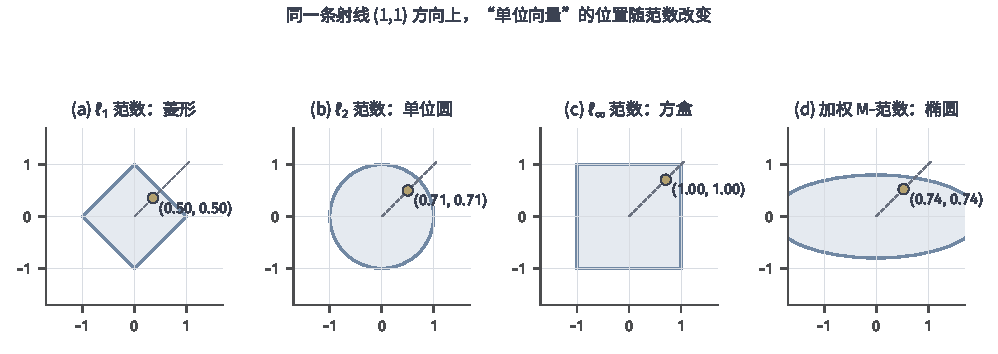
\includegraphics[width=169mm]{figures/01-mathematical-preliminaries-upper/02-linear-spaces/matplotlib/ls-norm-unit-balls/ls-norm-unit-balls.pdf}
  \caption{同一向量在不同范数下的“单位球”形状。左：$\ell_1$单位球为菱形（累加绝对偏差）；中：$\ell_2$单位球为圆（欧氏长度）；右：$\ell_\infty$单位球为正方形（最大坐标偏差）。同一个点$(1,1)$的范数依次为$2$、$\sqrt2$、$1$，单位球大小随口径而变，三者之间的倍数关系由正文的显式不等式给出。三图坐标尺度相同，为解析教学例。}
  \label{fig:ls-norm-unit-balls}
\end{figure*}

$p=1,2,\infty$的三角不等式可以直接验证；一般$p$需要下面的不等式。
\begin{theorem}[有限维Hölder不等式]
\label{thm:linear-algebra-holder}
设$1\leq p,q\leq\infty$且$1/p+1/q=1$（约定$1/\infty=0$），则$|\bm x^\top\bm y|\leq\lVert\bm x\rVert_p\lVert\bm y\rVert_q$。
\end{theorem}
\begin{proof}
先设$1<p,q<\infty$。Young不等式$uv\leq u^p/p+v^q/q$对$u,v\geq0$成立：$u>0$时令$t=v/u^{p-1}$，验证$1/p+t^q/q-t\geq0$，其最小值在$t=1$处为零；$u=0$时也成立。两向量非零时取$u_j=|x_j|/\lVert\bm x\rVert_p$、$v_j=|y_j|/\lVert\bm y\rVert_q$求和，得$\sum_j u_jv_j\leq1/p+1/q=1$，恢复尺度后用$|\bm x^\top\bm y|\leq\sum_j|x_j||y_j|$。零向量时两侧都为零；$p=1,q=\infty$时用$\sum_j|x_j||y_j|\leq(\max_j|y_j|)\sum_j|x_j|$，另一端点交换两者。
\end{proof}
对一般$p$，把$|x_j+y_j|^{p}\leq|x_j+y_j|^{p-1}(|x_j|+|y_j|)$求和后对两部分分别应用Hölder，得到
$\lVert\bm x+\bm y\rVert_p^p\leq(\lVert\bm x\rVert_p+\lVert\bm y\rVert_p)\lVert\bm x+\bm y\rVert_p^{p-1}$，非零时相除即得三角不等式（Minkowski不等式）。常用坐标范数之间还有直接界
\[
 \lVert\bm x\rVert_\infty\leq\lVert\bm x\rVert_2\leq\sqrt d\,\lVert\bm x\rVert_\infty,
 \qquad
 \lVert\bm x\rVert_2\leq\lVert\bm x\rVert_1\leq\sqrt d\,\lVert\bm x\rVert_2,
\]
右端两式分别来自$\sum_jx_j^2\leq d\max_jx_j^2$与Cauchy--Schwarz不等式。维数增大时$\sqrt d$不能在误差预算中忽略。

分组误差要先固定分组方式，例如以行为组的混合范数
$\lVert\bm A\rVert_{p,q}=(\sum_i\lVert\bm A_{i,:}\rVert_p^q)^{1/q}$，内层衡量组内、外层汇总各组。允许非零对象也具有零大小、但保留齐次性与三角不等式的尺度称为\term{半范数}（seminorm），它给出伪距离：例如只读取截距的仿射函数尺度$p(f_{a,b})=|a|$忽略全部斜率方向，相同截距的不同函数距离为零。把零方向归并为同一元素后得到的商范数，在讨论点到子空间的距离时给出（第~\ref{sec:ls-quotient-norms}节）。

\subsection{矩阵范数}
\label{sec:ls-matrix-norms}

矩阵有两种“大小”口径：Frobenius范数描述数表本身有多大；误差分析更关心它作为变换最坏把输入放大多少倍。
\begin{definition}[由向量范数诱导的矩阵范数]
\label{def:matrix-analysis-induced-norm}
给定输入范数$\lVert\cdot\rVert_\alpha$和输出范数$\lVert\cdot\rVert_\beta$，\term{诱导矩阵范数}（induced matrix norm）为
\[
 \lVert\bm A\rVert_{\alpha\to\beta}
 =\sup_{\bm x\neq0}\frac{\lVert\bm A\bm x\rVert_\beta}{\lVert\bm x\rVert_\alpha}.
\]
两端采用同一类$p$范数时简写为$\lVert\bm A\rVert_p$。
\end{definition}

\paragraph{诱导矩阵范数}

由定义直接得$\lVert\bm A\bm x\rVert_\beta\leq\lVert\bm A\rVert_{\alpha\to\beta}\lVert\bm x\rVert_\alpha$，诱导范数就是这一不等式中最小的常数。标准坐标下两个诱导范数可直接读取：
\[
 \lVert\bm A\rVert_1=\max_j\sum_i|a_{i,j}|,\qquad
 \lVert\bm A\rVert_\infty=\max_i\sum_j|a_{i,j}|.
\]
第一式由$\lVert\bm A\bm x\rVert_1\leq\sum_j|x_j|\lVert\bm A_{:,j}\rVert_1$得到上界，在最大绝对列和对应的坐标向量上达到；第二式的上界同理，取输入各坐标为对应行元素的符号即达到。诱导$2$范数也称\term{谱范数}（spectral norm），$\lVert\bm A\rVert_2=\sup_{\lVert\bm x\rVert_2=1}\lVert\bm A\bm x\rVert_2$；对每行用CS不等式得$\lVert\bm A\bm x\rVert_2\leq\lVert\bm A\rVert_{\mathrm F}\lVert\bm x\rVert_2$，故它有限且$\lVert\bm A\rVert_2\leq\lVert\bm A\rVert_{\mathrm F}$，其奇异值表达在第~\ref{sec:ls-svd}节推导。对一般的范数对，比值有界且上确界在某个方向达到，由第~\ref{sec:ls-error-scale-comparison}节的范数等价与极值定理保证。图~\ref{fig:ls-induced-norm-action} 把单位圆被拉成椭圆后的最长轴读作最大放大倍数。
\begin{figure*}[htbp]
  \centering
  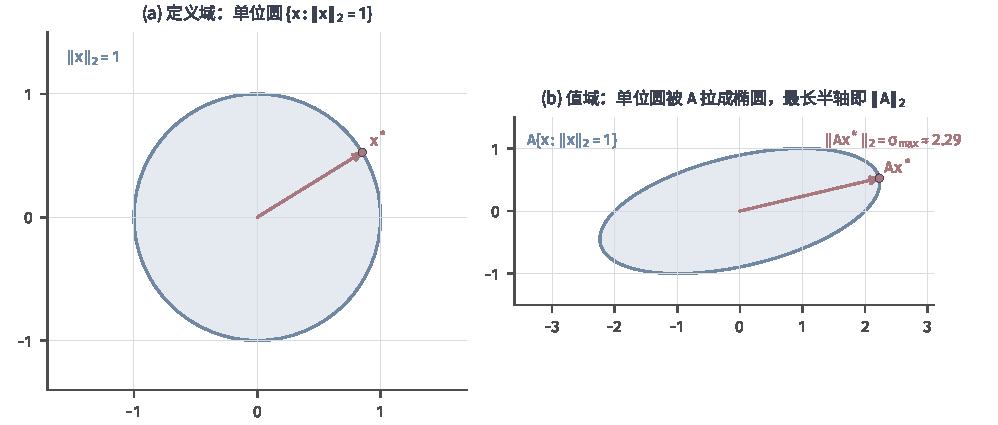
\includegraphics[width=169mm]{figures/01-mathematical-preliminaries-upper/02-linear-spaces/matplotlib/ls-induced-norm-action/ls-induced-norm-action.pdf}
  \caption{诱导矩阵范数衡量最坏放大倍数。左：单位圆$\lVert\bm x\rVert_2=1$；中：同一线性作用$\bm A$把单位圆映成椭圆；右：椭圆上最长的轴给出$\lVert\bm A\rVert_2=\max_{\lVert\bm x\rVert_2=1}\lVert\bm A\bm x\rVert_2$，箭头指示最大放大方向。数值由$\bm A$的教学构造直接得到，是解析例。}
  \label{fig:ls-induced-norm-action}
\end{figure*}

Frobenius范数从另一个角度累计作用：
\[
 \lVert\bm A\rVert_{\mathrm F}^2
 =\sum_j\lVert\bm A\bm e_j\rVert_2^2
 =\sum_{i,j}a_{i,j}^2,
\]
它是所有标准输入方向的总平方输出，而非一次最坏输入。对$\bm A=\begin{smallmatrix}1&1\\0&1\end{smallmatrix}$，$\lVert\bm A\rVert_1=\lVert\bm A\rVert_\infty=2$、$\lVert\bm A\rVert_{\mathrm F}=\sqrt3$，不同口径的数值不必相同。

中间空间范数匹配时，连续应用两次界得到次乘性
\[
 \lVert\bm A\bm B\rVert_{\alpha\to\gamma}
 \leq\lVert\bm A\rVert_{\beta\to\gamma}
 \lVert\bm B\rVert_{\alpha\to\beta}.
\]
逐列应用诱导范数界，转置后对列重复同一论证，得到混合界
\begin{equation}
 \lVert\bm A\bm B\rVert_{\mathrm F}
 \leq\lVert\bm A\rVert_2\lVert\bm B\rVert_{\mathrm F},
 \qquad
 \lVert\bm A\bm B\rVert_{\mathrm F}
 \leq\lVert\bm A\rVert_{\mathrm F}\lVert\bm B\rVert_2.
 \label{eq:matrix-analysis-mixed-submultiplicativity}
\end{equation}
其中$\lVert\bm B^\top\rVert_2=\lVert\bm B\rVert_2$可由
$\lVert\bm B\rVert_2=\max_{\lVert\bm x\rVert_2=\lVert\bm y\rVert_2=1}|\bm y^\top\bm B\bm x|$交换两向量得到。结合$\lVert\bm A\rVert_2\leq\lVert\bm A\rVert_{\mathrm F}$，Frobenius范数也次乘。

\subsection{距离与夹角}

范数诱导的距离$d(\bm x,\bm y)=\lVert\bm x-\bm y\rVert$满足非负、对称与三角不等式；非零向量的夹角已由CS不等式在第~\ref{sec:ls-inner-products}节定义。更换范数只改变距离口径，不改变两点是否重合。

比较两个方向时先把各自归一化到单位长度，消除整体缩放：$\bm x$与$c\bm x$（$c\neq0$）是同一方向，$\langle\bm x/\lVert\bm x\rVert,\bm y/\lVert\bm y\rVert\rangle$才只反映角度。两个子空间之间的夹角以各自单位向量之间的最小夹角为起点定义，其计算与敏感度在后续分析章节展开。尺度约定不同（例如一边用$\ell_2$、一边用$\ell_1$又不归一）时，比较结果没有意义，因此先统一度量口径再谈远近。

\subsection{对偶范数}
\label{sec:ls-dual-norms}

\paragraph{对偶范数}

误差$\bm r$只知道落在某个范数球内时，一次线性读取$\bm z^\top\bm r$最多变化多少，由下面的量回答。
\begin{definition}[对偶范数]
\label{def:linear-algebra-dual-norm}
给定$\mathbb R^d$上的范数，相对于标准坐标配对的\term{对偶范数}（dual norm）为
\begin{equation}
 \lVert\bm z\rVert_*=\sup_{\lVert\bm r\rVert\leq1}|\bm z^\top\bm r|.
 \label{eq:linear-algebra-dual-norm-definition}
\end{equation}
\end{definition}
它满足范数公理：线性读取满足三角不等式与齐次性，非零$\bm z$总能读取某个坐标得到非零值。对$\ell_p$范数，下面直接构造达到上确界的$\bm r$；一般范数下上确界同样可以取到（第~\ref{sec:ls-error-scale-comparison}节）。图~\ref{fig:ls-dual-norm-unit-ball} 把这个最大值画成支撑线最后接触单位球的位置。

\begin{figure}[!htb]
  \centering
  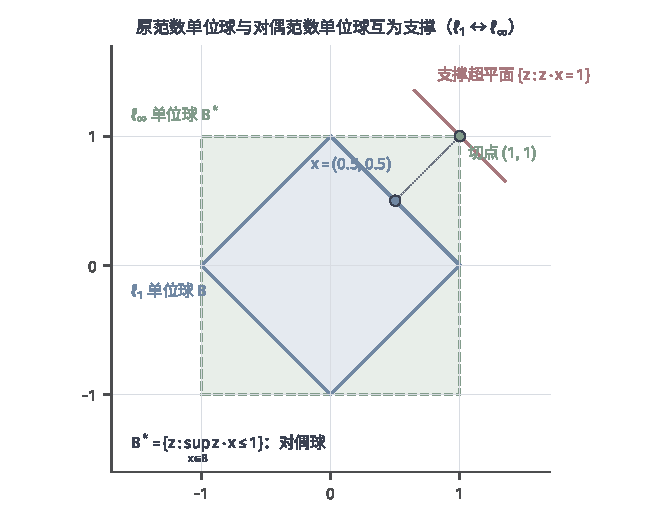
\includegraphics[width=112mm]{figures/01-mathematical-preliminaries-upper/02-linear-spaces/matplotlib/ls-dual-norm-unit-ball/ls-dual-norm-unit-ball.pdf}
  \caption{对偶范数的几何：在原范数单位球$\lVert\bm r\rVert\leq1$上求线性读取$\bm z^\top\bm r$的最大值。左：原单位球（灰色）与读取方向$\bm z$；右：支撑直线最后接触单位球处给出$\lVert\bm z\rVert_*=\max_{\lVert\bm r\rVert\leq1}|\bm z^\top\bm r|$。对偶单位球（虚线）与原单位球互为极体，为解析教学例。}
  \label{fig:ls-dual-norm-unit-ball}
\end{figure}

Hölder不等式给出$\ell_p$单位球上的上界$\lVert\bm z\rVert_q$，且上界可达到：$1<p<\infty$时取$r_j=|z_j|^{q-1}\operatorname{sgn}(z_j)/\lVert\bm z\rVert_q^{q-1}$；$p=1$时把单位预算放在$|z_j|$最大的坐标；$p=\infty$时逐坐标取$r_j=\operatorname{sgn}(z_j)$。因而
\begin{equation}
 (\lVert\cdot\rVert_p)_*=\lVert\cdot\rVert_q,\qquad \frac1p+\frac1q=1,
 \label{eq:linear-algebra-lp-duality}
\end{equation}
并对$\rho\geq0$有
\begin{equation}
 \max_{\lVert\bm r\rVert_p\leq\rho}|\bm z^\top\bm r|
 =\rho\lVert\bm z\rVert_q.
 \label{eq:linear-algebra-linear-perturbation-duality}
\end{equation}
例如$\bm z=(2,-1)^\top$、$|r_j|\leq0.01$时最大变化为$0.03$，由$\bm r=(0.01,-0.01)^\top$达到。图~\ref{fig:linear-algebra-dual-unit-balls} 固定同一次读取，显示预算形状怎样改变最坏方向。
\begin{figure*}[htbp]
  \centering
  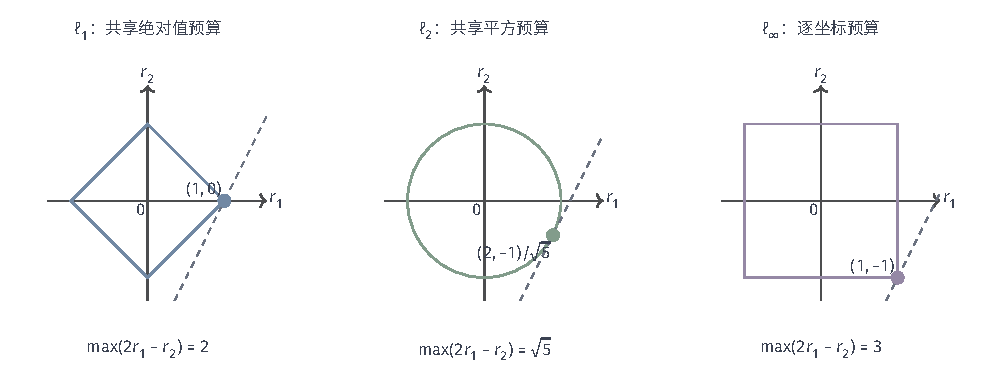
\includegraphics[width=168.998mm]{figures/01-mathematical-preliminaries-upper/02-linear-spaces/tikz/linear-algebra-dual-unit-balls/figure.pdf}
  \caption{同一线性读取$2r_1-r_2$在$\ell_1$、$\ell_2$、$\ell_\infty$单位球上的最大值依次为$2$、$\sqrt5$、$3$。虚线为最后接触可行集的支撑直线，点为最大化方向。三图坐标尺度相同，均为解析教学例；改变允许误差的形状会改变误差常数。}
  \label{fig:linear-algebra-dual-unit-balls}
\end{figure*}

加权长度$\lVert\bm r\rVert_{\bm M}=\sqrt{\bm r^\top\bm M\bm r}$的对偶范数由逆矩阵给出：误差按$\bm M$计量时，读取方向要按$\bm M^{-1}$计量。
\begin{theorem}[加权对偶范数]
\label{prop:ls-weighted-dual-norm}
设$\bm M$对称正定，则范数$\lVert\cdot\rVert_{\bm M}$相对于标准坐标配对的对偶范数为
\[
 \lVert\bm z\rVert_{\bm M,*}
 =\sup_{\bm r^\top\bm M\bm r\leq1}\bm z^\top\bm r
 =\sqrt{\bm z^\top\bm M^{-1}\bm z}.
\]
\end{theorem}
\begin{proof}
取可逆配方因子$\bm M=\bm L^\top\bm L$（定理~\ref{thm:ls-gram-factor}），令$\bm w=\bm L\bm r$，约束化为$\bm w^\top\bm w\leq1$，目标化为$\bm z^\top\bm r=\bm z^\top\bm L^{-1}\bm w=(\bm L^{-\top}\bm z)^\top\bm w$。由欧氏情形$\sup_{\lVert\bm w\rVert_2\leq1}\bm a^\top\bm w=\lVert\bm a\rVert_2$（$\bm w=\bm a/\lVert\bm a\rVert_2$时取到），上确界为
\[
 \lVert\bm L^{-\top}\bm z\rVert_2
 =\sqrt{\bm z^\top\bm L^{-1}\bm L^{-\top}\bm z}
 =\sqrt{\bm z^\top\bm M^{-1}\bm z},
\]
其中$\bm L^{-1}\bm L^{-\top}=(\bm L^\top\bm L)^{-1}=\bm M^{-1}$。
\end{proof}

把约束中的$\bm r$按比例缩放，定理也可写成$\bm z^\top\bm M^{-1}\bm z=\sup_{\bm r\neq\bm0}(\bm z^\top\bm r)^2/(\bm r^\top\bm M\bm r)$。由这一极值写法立即得到正定矩阵求逆的序反转。
\begin{theorem}[正定求逆的序反转]
\label{cor:ls-inverse-order-reversal}
若$\bm M_1\preceq\bm M_2$都正定，则$\bm M_2^{-1}\preceq\bm M_1^{-1}$。
\end{theorem}
\begin{proof}
对任意$\bm z$，由$\bm r^\top\bm M_1\bm r\leq\bm r^\top\bm M_2\bm r$，分母较小者比值较大：
\[
 \bm z^\top\bm M_2^{-1}\bm z
 =\sup_{\bm r\neq\bm0}\frac{(\bm z^\top\bm r)^2}{\bm r^\top\bm M_2\bm r}
 \leq\sup_{\bm r\neq\bm0}\frac{(\bm z^\top\bm r)^2}{\bm r^\top\bm M_1\bm r}
 =\bm z^\top\bm M_1^{-1}\bm z.
\]
\end{proof}
原度量增大时，对偶度量缩小。这是两个对称矩阵之间的序关系，不是逐元素不等式。

\section{伴随}
\label{sec:ls-adjoints}

矩阵转置把作用从输出端搬回输入端，但“搬运”依赖所选配对。内积空间中这个搬运者称为伴随；它与代数对偶中的转置、与求解复原的逆是三个不同对象。

\subsection{定义与性质}

\paragraph{内积伴随的定义}

设$T:V\to W$是两个有限维实内积空间之间的线性映射。若存在$T^\star:W\to V$使
\begin{equation}
 \langle T\bm x,\bm y\rangle_W=\langle\bm x,T^\star\bm y\rangle_V
 \label{eq:ls-adjoint-pairing}
\end{equation}
对所有$\bm x\in V$、$\bm y\in W$成立，则$T^\star$称为$T$的\term{伴随}（adjoint）。
\label{def:linear-algebra-adjoint}

伴随总存在且唯一。取$V,W$的基，把两边的内积写成$\langle\bm x,\bm x'\rangle_V=\bm x^\top\bm M_V\bm x'$、$\langle\bm y,\bm y'\rangle_W=\bm y^\top\bm M_W\bm y'$，其中$\bm M_V,\bm M_W$是基的Gram矩阵，对称正定因而可逆；设$T$的矩阵为$\bm A$，所求伴随的矩阵为$\bm B$。式~\eqref{eq:ls-adjoint-pairing}要求$(\bm A\bm x)^\top\bm M_W\bm y=\bm x^\top\bm M_V\bm B\bm y$对所有$\bm x,\bm y$成立，即$\bm A^\top\bm M_W=\bm M_V\bm B$，它有唯一解
\begin{equation}
 \bm B=\bm M_V^{-1}\bm A^\top\bm M_W.
 \label{eq:ls-weighted-adjoint}
\end{equation}
标准内积下$\bm M_V,\bm M_W$都是单位矩阵，伴随矩阵就是$\bm A^\top$；两边权重不同时，伴随既不是单纯转置，也不是转置再求逆。

伴随与组合的规则由配对定义逐项推出：
\[
 (T+S)^\star=T^\star+S^\star,\qquad
 (cT)^\star=c\,T^\star,\qquad
 (TS)^\star=S^\star T^\star,\qquad
 T^{\star\star}=T.
\]
复合伴随的次序与乘积转置一样反转；恒等映射的伴随是自身。图~\ref{fig:ls-adjoint-action-transfer} 把这种配对方向的搬回画成示意图。
\begin{figure}[!htb]
  \centering
  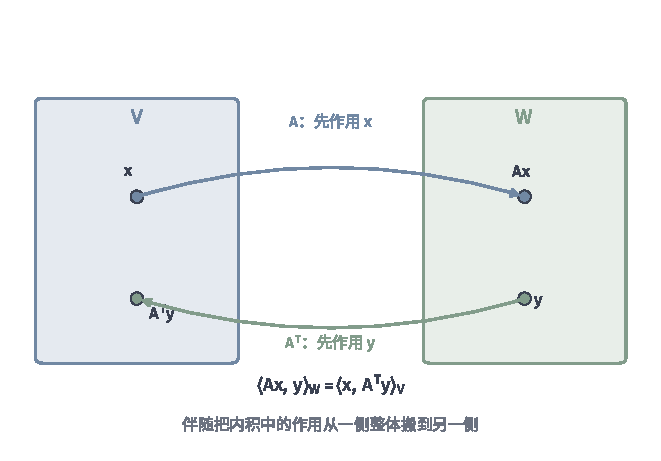
\includegraphics[width=112mm]{figures/01-mathematical-preliminaries-upper/02-linear-spaces/matplotlib/ls-adjoint-action-transfer/ls-adjoint-action-transfer.pdf}
  \caption{内积伴随把输出端的配对搬回输入端。左：$T:V\to W$把$\bm x$映成$T\bm x$，与$\bm y\in W$配对；右：伴随$T^\star:W\to V$把$\bm y$映回$T^\star\bm y\in V$，使$\langle T\bm x,\bm y\rangle_W=\langle\bm x,T^\star\bm y\rangle_V$。标准欧氏内积下$T^\star$就是转置，是配对方向的反转而非逆作用。箭头与空间为解析示意。}
  \label{fig:ls-adjoint-action-transfer}
\end{figure}

标准欧氏内积下伴随就是矩阵转置，因此转置是伴随在一种特定配对下的特例；更换加权内积后伴随一般不等于转置，见式~\eqref{eq:ls-weighted-adjoint}。第~\ref{sec:ls-dual-spaces}节从代数对偶出发的转置记录的是线性泛函的坐标变换，不需要内积。伴随也不是逆：逆把输出复原成输入，伴随只把读取方向换一侧。例如$2I$的伴随仍是$2I$，而逆为$\tfrac12 I$。

若$T^\star=T$，称$T$为\term{自伴}（self-adjoint），标准坐标下对应对称矩阵。若$Q^\star Q=I$，称$Q$为\term{正交}（orthogonal）作用：它保持内积$\langle Q\bm x,Q\bm y\rangle=\langle\bm x,Q^\star Q\bm y\rangle=\langle\bm x,\bm y\rangle$，在方阵情形下$Q^{-1}=Q^\star$。满足$TT^\star=T^\star T$的作用称为\term{正规}（normal）作用，自伴与正交都属于它；这些类别的谱性质在后续谱分解中展开，这里只给出定义。
